\chapter{Method} 

%The method chapter should describe in detail which activities you undertake to answer the research questions presented in the introduction, and why they were chosen. This includes detailed descriptions of experiments, surveys, computations, data analysis, statistical tests etc.

\section{Introduction}


As a background for the thesis, assume a threat actor is
 in a preliminary phase of an attack. The decision to initiate a phase of attack simulation is made, with the aim of gathering useful information in order to learn more about possible risks of being detected, as well as to gain some empirical background for the evaluation of possible consequences of a successful attack.
The potential outcome of the simulation may be used in order to prepare for attacking the actual infrastructure with attacks with a low attack detection probability and, to the best possible knowledge, with foreseeable consequences of the attack.

As described previously, the aim of the thesis is to investigate any observable effects of specific time delay attack simulations. Such simulations could be executed in a preparation phase, preparing for the execution of an actual time delay attack.

 \hl{Some papers} describes a number of varieties of the PTP delay attack, while \hl{other papers} describes the attack to have severe consequences to the \acrshort{sg} infrastructure. The primary goal of the actual attack is to stay undetected, while exposing the infrastructure under attack to an attack having the most severe consequences possible, while still avoiding detection.  
 


%For the \acrfull{wams} Security parts, a small number of surveys, as well as a collection of papers are investigated, covering  synchrophasor protocol attack vulnerabilities, highlithing some known side effects of successful synchrophasor protocol attacks. The introductory brief coverage of \acrshort{sg} security, is followed by a coverage of common synchrophasor protocols, focusing on attack vulnerabilities of the protocols covered. \\ 






%Several test cases utilising PMUs and PDCs



%In order to investigate, systems like mininet. \\ 


\section{Research Design}
%This section will inform the reader of the NATURE of your study. In other words, broadly speaking: are you aiming to describe a phenomena (descriptive design), are you aiming to explore a topic (exploratory design), are you looking to identify causal relationships between factors (causal design)?

%The aim of the thesis, is to present an overview of concepts, as well as to to provide examples from the literature related to the Smart Grid WAMS being vulnerable to attacks on the Synchrophasor protocols. 
In order to be able to observe the effects of exposing a \acrshort{pmu} to a time delay attack, the real attack is dependant on getting access to expensive equipment, like a \acrshort{pmu} as well as the interconnected infrastructure.
As previously discussed, a time delay attack on Synchrophasors imposes a high risk of causing damage to the infrastructure targeted.
Given the high potential for damage, a good option for visualising any potential effects a time delay might have on the values produced by a \acrshort{pmu} under attack, would be to simulate the attacks.
There exists a number of projects which utilises MATLAB and SIMULINK in order to model power grid components in general and, specifically, \acrshort{pmu}s.

My selected approach, however is to produce a SIMULINK model, using standard components from the Simscape Electrical addon to MATLAB/SIMULINK. The simulation produces pair-wise (original, delayed) PMU output values for each of the channels Magnitude, Angle and Frequency, making them available for comparison and further analysis. \hl{The analytic part could be one obvious candidate for further work.}

%
%Two identical copies of the PLL PMU is connected to a power source, one directly, the other via the delay function. The resulting output is pair-wise collected to one channel for each of the components Magnitude, frequenct

%In order to 

%Based on the findings of the initial literature study concerning vulnerabilities, the literature study continues providing potential scenarios for stealthy MiTM attacks on the synchrophasor transmission system, investigating the success of the attacks maximising side effects while minimising the probability of being detected.

As the final part of the thesis, a theoretical discussion, aiming to provide answers to the research questions, will be conducted.\\ 

%\textbf{TO DO:}
%\hl{As a experimental part of the thesis, possibilities of testing one or more detection and mitigation techniques might provide a contribution to the final discussion and conclusions based on my own experimental results}


\section{Research Methods}
As the thesis includes both a theoretical, as well as a more practical phase, the methods are dependant on the phase in question.
%Following the description of your research design, you should also devote a section to describing the research methods you applied during your study. Each design will provide you with many possibilities of methods to use.
\subsection{Theoretical phase}
As part of the introductory studies of the topic selected, a couple of searches on the NTNU literature search facilities returned a number of books, like \cite{BlumeStevenW2007Epsb} and \cite{kabalci2019smart}, covering introductory chapters on Power Grid and Smart Grid. The introductory chapters heavily relies on descriptions from relevant book chapters. 

\subsection{Practical phase}


In order to provide theoretical evidence on which to answer the research questions, a literature study will be conducted.
For any experimental results, experiments will be described, implemented and executed.

\section{Measurements}

%Once you clarified the method you used, it is time to explain exactly WHAT you measured (e.g. service quality, brand image, satisfaction, purchase intention) and HOW you measured

%Vulnerability to time-shift attacks are quantified by articles describing theoretical aspects of the mechanisms for the calculation of valid time-stamps, and the inherent tolerance level for calculation errors. 
%Modern Smart Grids require the time deviating from the correct time by a fraction of a millisecond. Specifically, according to \cite[p.  1953]{moussa2016security}, the allowed time deviation for a 50Hz electrical system\footnote{As used in Norway, for instance} must be within $\pm31.8\mu s$, in order to adhere to the 1$\%$ \acrfull{tve} requirement, as specified by the  IEEE C37.118 standard. \\ 


The simulations to be defined and executed provides examples of \acrlong{pmu} output, where two identical \acrshort{pmu}s are given a signal from a simulated power source as input. One of the PMUs are fed the original power source signal, whereas the other PMU is fed a delayed version of the original power source signal. The resulting PMU output measurements may be compared for similarity. 

Where possible, experimental investigations reported by articles selected will be provided as relevant examples, in order to support any discussion arguments for the purpose of reaching conclusions.  

\section{Sample}

%In this section you should detail (at least!) the population of your study, your sampling technique (which technique you used to select the people who took part in your study) and how you established your sample size.
The samples for my literature study will be papers relevant for the discussions, in order to provide answers to the research questions.\\ 

Any execution of experiments will provide experimental samples, with the aim of supporting discussions and conclusions.
The samples originating from the experiments, consists of:
\begin{itemize}
    \item Three channels of PMU output, denoted \textbf{Magnitude}, \textbf{Frequency} and \textbf{Angle} 
    \item Two arrays of numerical values for each channel of PMU output: One for the original signal, the other for the delayed signal. 
\end{itemize}
\section{Validity and Reliability}

%Now, here is a SUPER important section that 99\% get wrong(I completely made up this figure, simply because I want to convey a point!). Validity (that you measured what you intend to measure) and reliability (that the measurements used, such as your scales, are consistent and replicable) are two concepts that simply have to be addressed and have to do with your measurements.
In order to increase the validity and reliability, a number of articles will be included as the foundation for any conclusions. My personal selection of papers deemed relevant for my discussion, will be selected highlighting on articles being included as relevant articles by survey papers, as well as papers gaining a high relevance score on literature search sites.\footnote{... like the NTNU ORIA site (\url{https://innsida.ntnu.no/litteratur}).} Another selection criteria aiming to increase validity and reliability will be a focus on selecting articles receiving a high number of quotations ratings on sites like Google Scholar. %First and foremost, though, a sound and critical validation of the relevance for the questions at hand is still mandatory. \\  



For the experimental parts, my project is utilising a selection of PDC and PMU simulator packages. In order to validate the phasor data generated, the included validation capabilities of the simulator packages are utilised. 
\subsection{Validation of the model}
A experiment of running the simulation with a delay leve of 0, could serve two purposes:
\begin{itemize}
    \item Validation of the delay function
    \item Validation of the two copies of the PMU as being identical.
\end{itemize}
As a hyphothesis, running the simulation with a delay of zero should produce identical channel-wise output.

A $d=0$ test result  producing identical output for the who PMUs , would increase the 
confidence of the model both being valid and reliable.

Another criterion for a valid model would be for the data to show alterations which could be explained by a change of delay level.



\section{Infrastructure used during experiments }
\hl{A selection of a relevant infrastructure for experiments will be made according to  specific needs and availability.  }\\ 

In order to provide practical results on which to base the discussions and conclusions, the following tools will be utilised;

\begin{itemize}
%    \item The iPMU suite, including iPDC, iPMU and PMUSimulator, running on virtual Ubuntu Linux instances
%    \item The pyPMU suite, including tinyPDC, tinyPMU and , running on virtual Ubuntu Linux instances \cite{vsandi2015python}, \cite{vsandi2016pypmu}
    %\item A SIMULINK model, downloaded from \textbf{URL} is used as the basis for the simulations.
    \item MATLAB, R2023a, with SIMULINK added, is used for running the simulation. 
    \item Simscape Electric, and its dependency Simscape, are required in order to build, and run, the simulations.
    \item The Simulation is executed by running a MATLAB script.
    \item A Windows 10 laptop is being used for the simulations
    
 %   \item mininet will be utilised for networking
 %   \item Wireshark will be utilised for synchrophasor packet analysis
 %   \item Python will be utilised in order to visualise the results

\end{itemize}

%\section{Instruments or Equipment}

%Sometimes, especially in causal studies when researchers are developing experiments, it is important to detail the instruments or equipment that were used in the study.



\section{Simulating a Time Delay attack}



\subsection{Scenarios}

For the experimental part of my thesis, a number of attack scenarios will be required. The aim is to investigate various attack vectors which might be used by a sophisticated man-on-the-side threat actor in order to execute an attack while staying undetected. 

\subsection{Assumptions} 

A number of assumptions is stated, in order to narrow the scope of the thesis:

\begin{itemize}
    
\item \textbf{Attacker Policy} 
A sophisticated threat actor would most likely want to avoid detection by anyone protecting the targeted infrastructure.
Therefore, executing an attack which may be detected should be avoided at all costs.
As a consequence, any decisions related to actually executing the attack should be as a result of promising results following a stealthiness assessment process. Simulations of possible effects could be part of the stealthiness assessment process. 

\item \textbf{Attack Prerequisites} 
A stealthy attack with small impact is preferred over an attack having more severe impacts, at a higher risk of detection.
The ideal attack would be an attack having maximal impact on the target, while the risk of detection being minimal. 


\item \textbf{Attack Design Policy} 
A part of the challenge would be to design an attack producing a high impact on the target, while staying undetected.
\end{itemize}
\subsection{Approach Selected for the Attack} 
One possible solution could be to determine the minimal efforts needed in order to execute an attack with a high probability of producing the effects desired, while keeping the attack detection probability low.




\subsection{Definition of scenarios}
In order to provide experimental results in order to answer the Research Questions stated, a number of attack scenarios are defined.
The main method of simulation would be a delayed forwarding of values, where a specified delay $d$ is applied to the PMU input, replacing any sample $s(i)$ with the sample value $s(i-d)$, simulating clock drift, producing effects similar to a \acrlong{tda}.

The simulation could be performed using a number of delay functions. In order to investigate some specific effects the following characteristics are selected:



\begin{enumerate}
\item In order for the model to stabilise\footnote{The PMU needs some samples of input before being able to stabilise the output values.}, data used for visualisation does not include the first second of the simulation ($t < 1$).
\item In order to be able to conclude on the effect of delay cancellation, each simulation is executed  with a delay level of 0 for the next second ($1 < t < 2$). 
\item  The instant attack involves raising the delay level instantly to a level $d > 0,  d \in \mathbb{N}$, at the time $t = 2$
\item  The step-wise attack involves raising the delay level in steps of one each second from $t = 2$ until reaching the level $d$ at $t = 1+d$.  
\item  In order to be able investigate any effects of attack cancellations, the targeted PMU is exposed to a delay attack for a limited time, thus reducing the delay level $d$ to $0$ before reaching the last second of the pre-set simulation running time.   
\end{enumerate}
    


\subsection{Attack Implementation}
%The attacks would be implemented as MATLAB functions executing attacks on targets implemented as SIMULINK simulations. The various scenarios would  be required to be sufficiently similar to be implemented as variations of a single attack framework, in order to avoid the need of creating more than a single attack framework.     

%In order to prepare for attacks, a plan might be to implement the techniques described in \cite{gilad2014off}.



%\textbf{\cite{barreto2016undetectable} proves the requirement of exposing more than two PMUs to a delay attack, for the attack to be undetectable.}




A number of physical investigations related to the effects of any intended attacks on the intended targets, would increase the knowledge of a potentially complex target, increasing the probability of staying undetected during the attack. In order to avoid exposing expensive and critical power system infrastructure to physical damage or downtime,\footnote{In a test lab environment, downtime could be acceptable, whereas the risk of physical damage of typically expensive equipment may be too high, at least not in the initial phases of investigations.} such practical investigations would preferably be performed in a simulation environment.

\section{Creating a Simulation environment}

This approach could be taken by a threat actor during a phase of investigations in the preparation of the actual attack, for the purpose of learning more about the possible consequences of performing intended actions on the intended target. One of the most important priorities of the threat actor, is to stay undetected for as long as possible. Simulations are designed in order to investigate the selected attack scenarios. The planned attack is implemented using a combination of Simulink and MATLAB. The execution of each simulation will produce corresponding graphs, illustrating any visible effects the attack may have on the system, by analytically comparing the output produced by the attack, with the alternative output of the unmodified, and correct Synchrophasor signal corresponding to  a situation of no attack being performed.

\subsection{Modelling a PMU}

As the plan of the threat actor is to expose  a number of \acrshort{pmu}s to a time  delay attack, the plan is to build a model of a \acrshort{pmu}, allowing the model to be run while altering any time stamp values required, in order to investigate any observable effects on the output from the \acrshort{pmu}.
 \begin{figure}[ht]
\centering
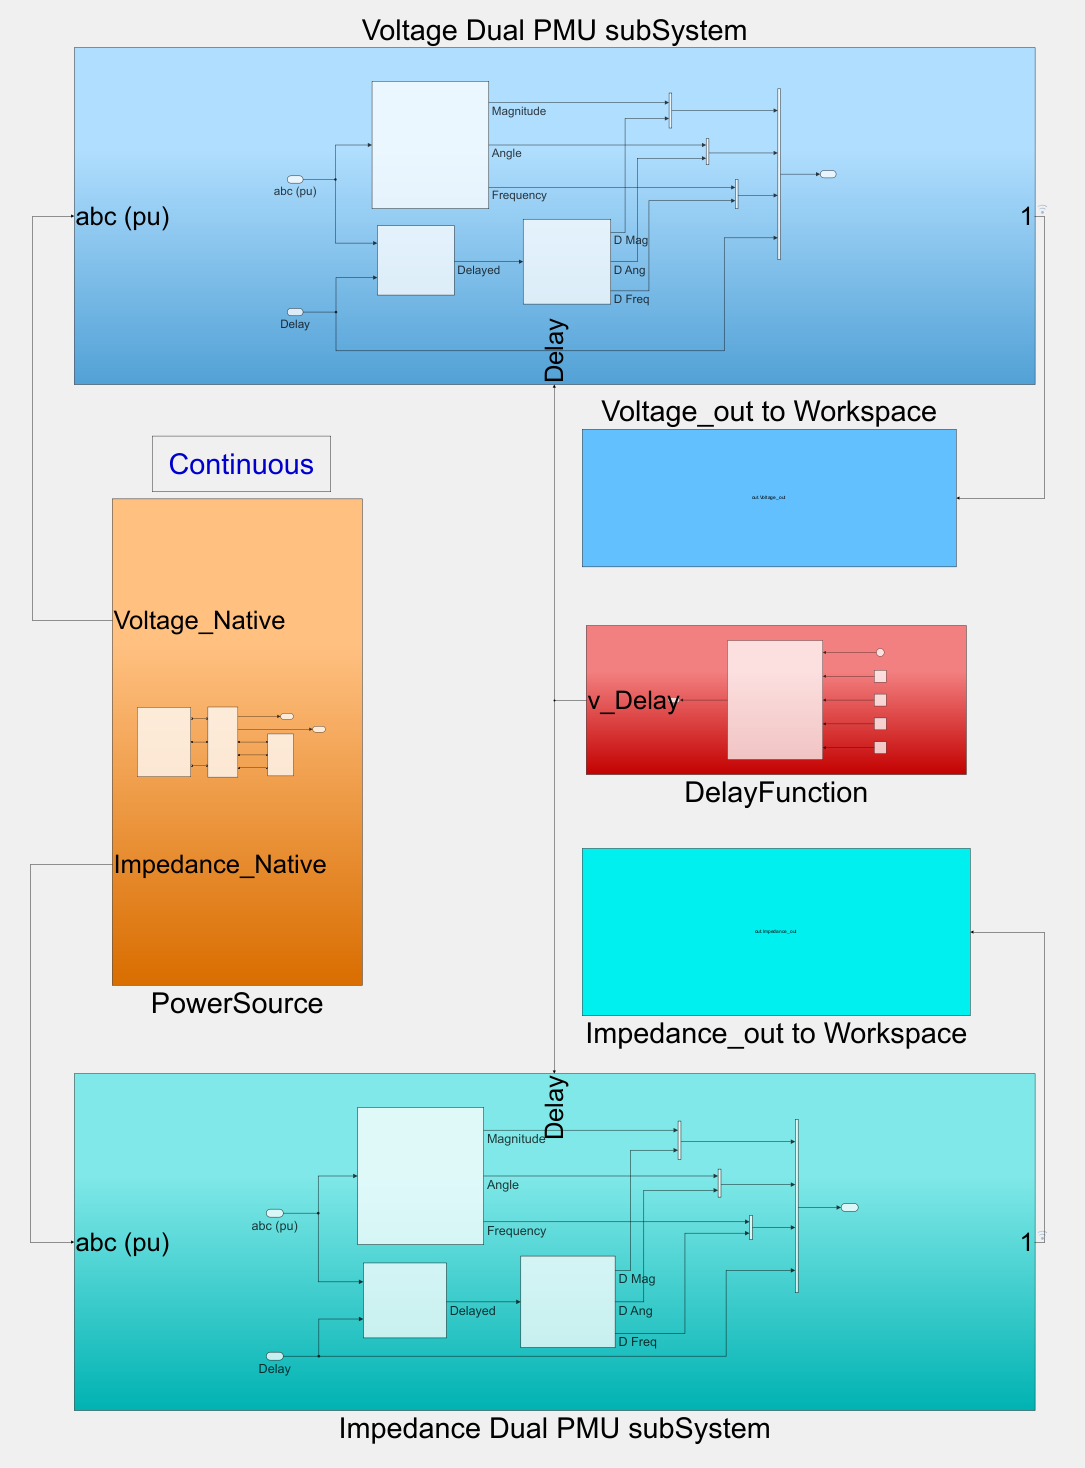
\includegraphics[width=0.9\textwidth]{figures/pmuSIM-overview.png}
\caption[PmuSIM SIMULINK model]{A SIMULINK model for the simulation of PMU Time Delay Attacks.}

\end{figure}


\subsubsection{The PowerSource subsystem}

 \begin{figure}[ht]
\centering
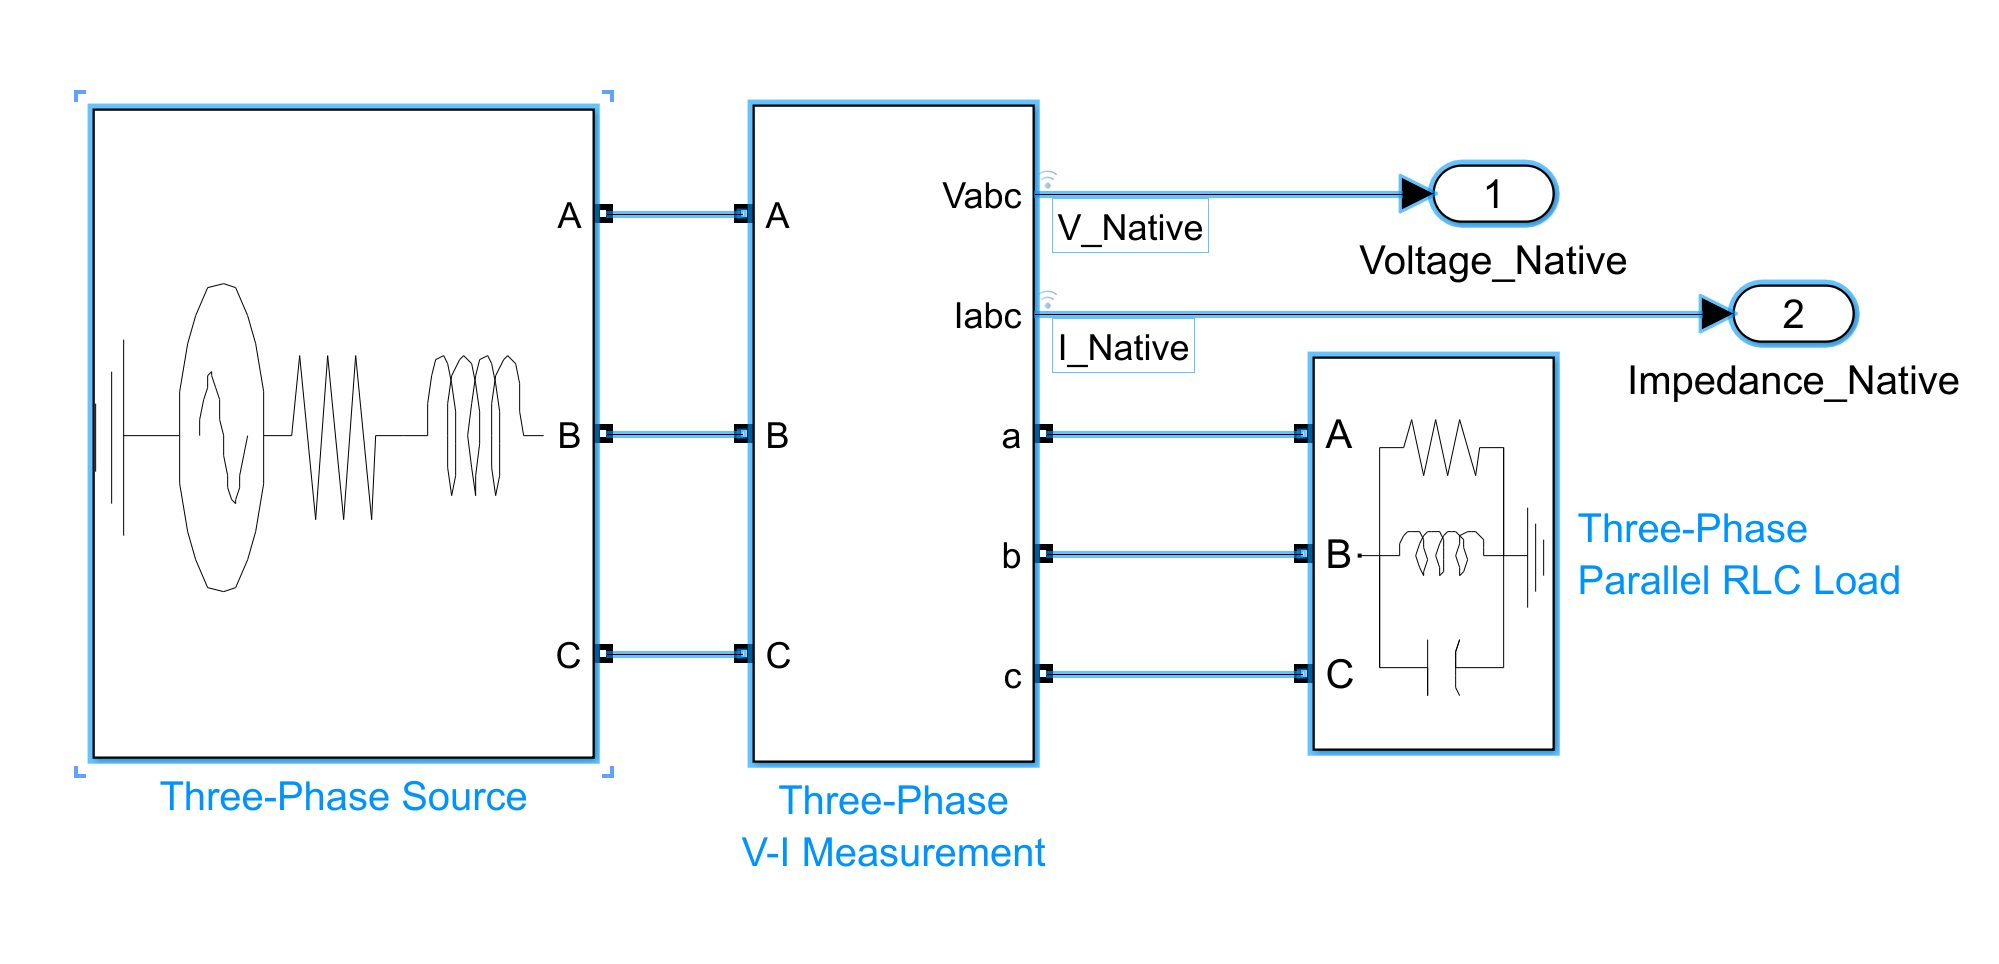
\includegraphics[width=0.9\textwidth]{figures/PowerSourceSubsystem.png}
\caption[PowerSource SIMULINK subsystem]{PowerSource: Generating  V and I PMU Input to DualPMU.}

\end{figure}

\subsubsection{The DualPMU subsystem}

 \begin{figure}[ht]
\centering
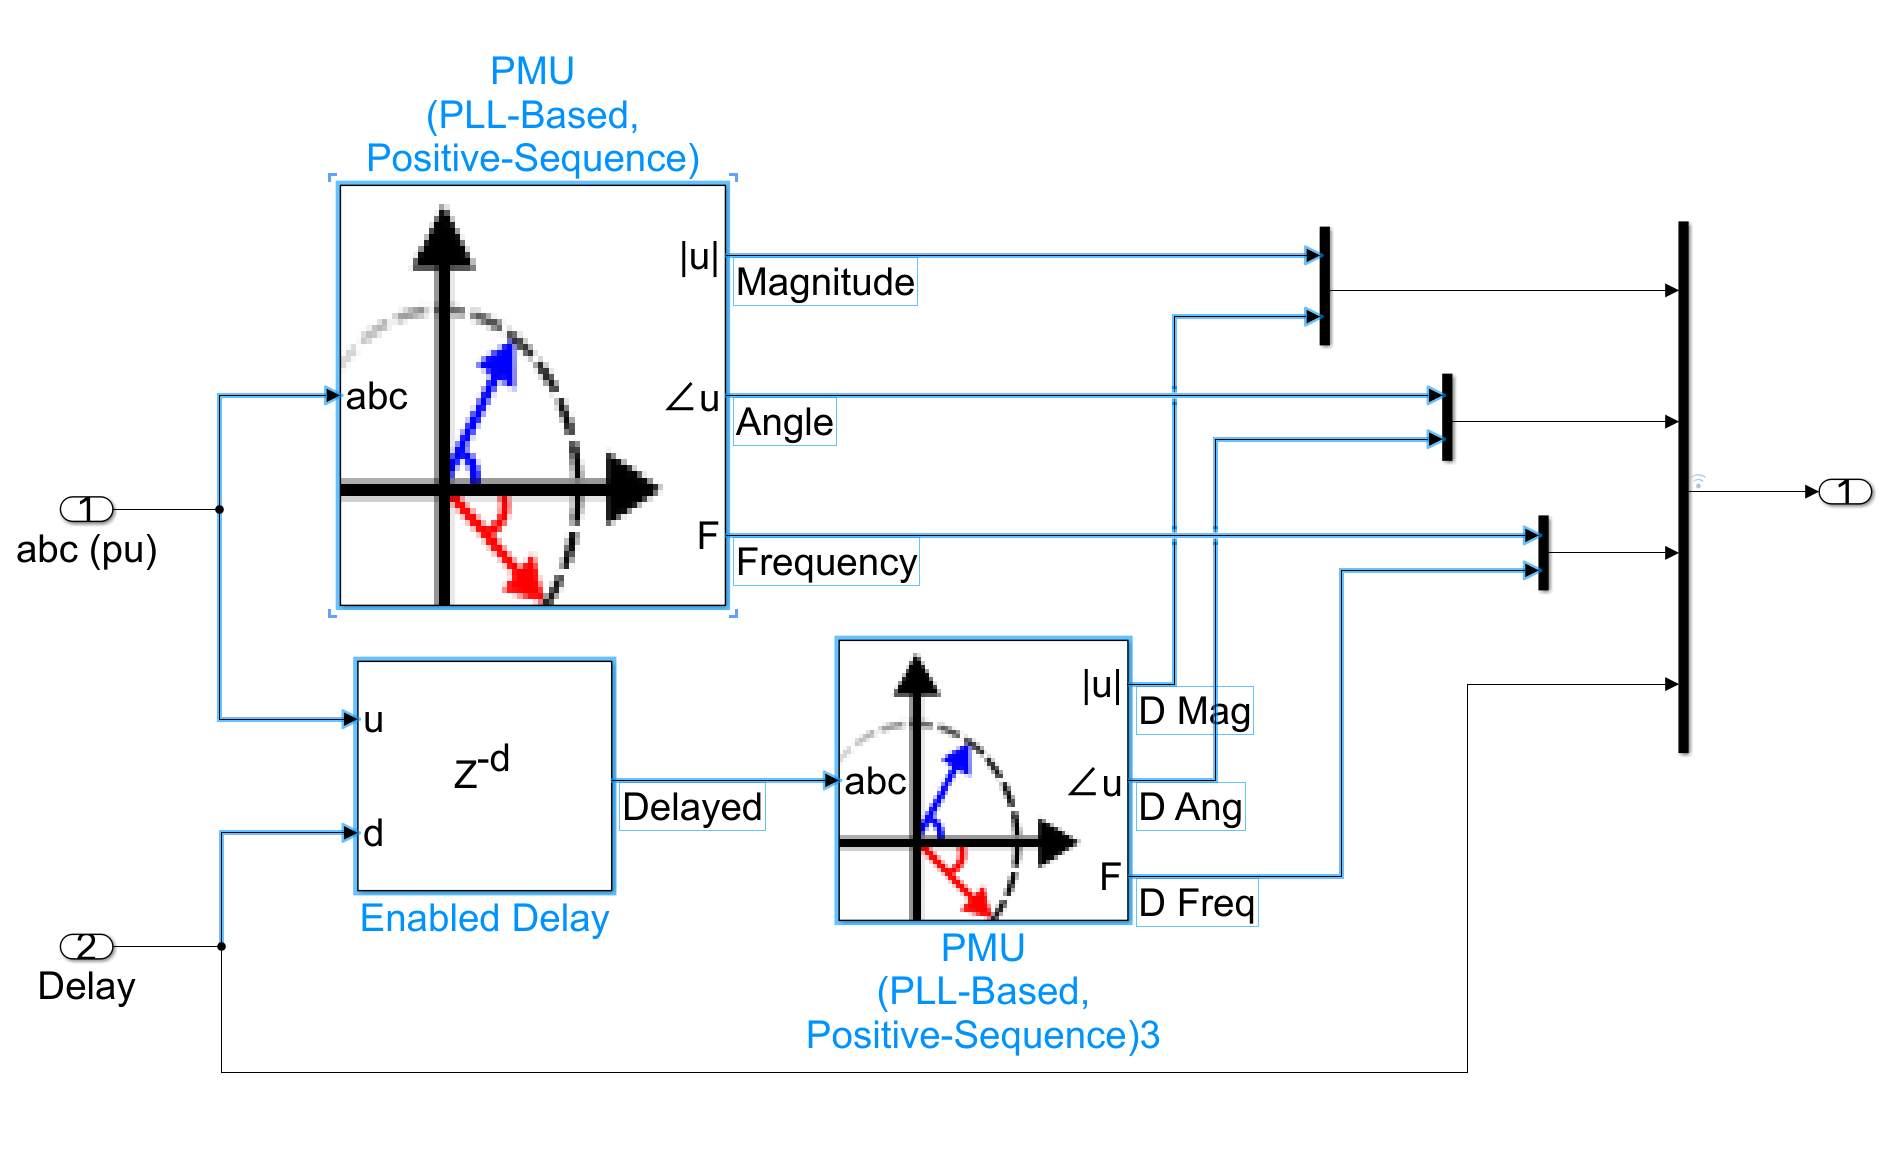
\includegraphics[width=0.9\textwidth]{figures/DualPMUsubsystem.png}
\caption[DualPMU SIMULINK subsystem]{DualPMU: Generating PMU output from V or I from PowerSource.}

\end{figure}



\subsection{Experimental Procedure}
%\textbf{TO DO:} \textit{Describe experimental procedure, dependant on experiments and experimental environment selected.}.
In order to complete one iteration of the simulation, each step should be completed, as required.
\begin{enumerate}
    \item Start Matlab
    \item Open a MATLAB script, named \textbf{PMUsimScript.m}.
    \item Inspect and modify a selection of variables, and execute the script for each run. The script will produce:
    \begin{enumerate}
    \item Output data logged to workspace according to the model.
    \item For each variation, a numeric comparison, followed by a corresponding colored (Green/Red) similarity classification.
    \item One combined figure showing original and delayed signal, as well as one figure for each of the PMU components "Angle", "Frequency" and "Magnitude".
    \item The figures are stored as specified in the MATLAB script.
    \end{enumerate}
    \item Planned analysis is to be determined, using component output generated. 
\end{enumerate}
Assumptions: 
Focus on a few optional tolerance levels. One Option: Assume a similarity of 0.95 to be hardly detectable.  
\begin{itemize}
    \item Use the lowermost drawings appearing in each component output generated for graph comparisons.
    \item Visually inspect the green portion, indicating tolerable difference as well as any red portions.
    \item The graphs may provide indications on attack stealthiness, by no, (or minimal) red portions in the lower drawing. 
    \item Tolerance levels: $1\% (0.01)$, $5\% (0.05)$ and $10\% (0.1)$ For now $1\%$ is covered.
\end{itemize}

\begin{enumerate}
    \item The green portion of the line indicates signal similarity, indication periods with a low probability of attack detection.
    \item The red portion of the graph is to be interpreted as time periods where the attack detection risk is too high for the attack to remain stealthy for lengthy periods of time.

\end{enumerate}
\subsection{Definition of Experiments} \label{sec:ExpDef}

%As discussed in an \textbf{Earlier Chapter}, according to \textbf{SELECTED PAPERS}, the \acrshort{sg} \acrshort{se} systems analysed would detect attacks producing signal differences of various levels of similarity. %around $10-15\%$ similarity.





The experiments will focus on various levels of assumed detection thresholds.

%My experiments will cover a selection of attack strategies for the selection of threshold levels of $1\%$, $5\%$ and $10\%$ similarities.

\begin{enumerate}
    \item \textbf{Immediate delay} Square pulse signal: Starting off, turning constant-delay on,  before dropping to 0 before simulation end. 
    \item \textbf{Step-wise delay} Increasing to delay level specified, in step-wise increse of delay level by one each second, before dropping to 0 before simulation end. 
    %\item Increasing delay, drop to 0 before simulation end
\end{enumerate}

Additonally, the  \textbf{No delay attack}, running the simulation on a constant delay level of $0$ for the entire duration of the simulation, will be executed in order to produce output for model validation purposes. 

\hl{The simulations need re-run}
%The current figures of chapter \ref{chap:Results} are produced by exposing the PMU to a variety of \textbf{d\_mode}s, as well as a selection of delay levels.



%The experiments, therefore, will focus on levels of delay of 0.1 to 0.15. For each level, the analysis will focus on various attack strategies, reaching the delay level in 1,2,3 and 4 steps, before keeping the delay for a total duration of  5 to 15 seconds.

%The experiments will be performed utilising \acrshort{pmu} simulation software, utilising available verification tools to ensure the compliance with established standards like the <--->
%The plan is to recreate experiments performed by <----> in a live environment, utilising  In order to test mitigation, mininet will be utilised

%Generate PMU data utilising simulators verified for compliance


%Utilise SADF \cite{SADF-framework} in MATLAB.

%Once again, in case you are running a causal study and an experiment, it is important to detail the experimental procedure.

%Explain, to the reader for example, what was the experimental task (what did the participants have to do?), the extraneous variables that were controlled (variables of the environment that could affect the cause and affect relationship).


